\documentclass[12pt,fleqn]{article}\usepackage{../../common}

\begin{document}
Yanl�l�k-Varyans Dengesi  (Bias-Variance Trade-off)

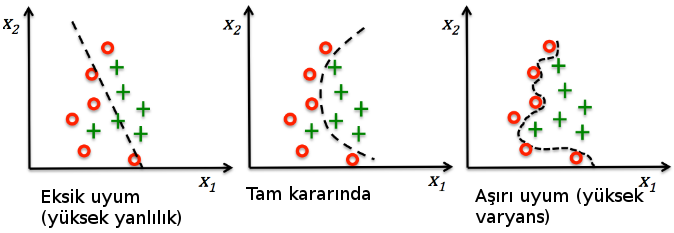
\includegraphics[width=30em]{biasvar_01.png}

\begin{minted}[fontsize=\footnotesize]{python}
from sklearn.svm import SVC
from sklearn.naive_bayes import GaussianNB
from sklearn import linear_model
from sklearn import ensemble
from sklearn.model_selection import ShuffleSplit
from sklearn.datasets import load_digits
import lcurve

digits = load_digits()
X, y = digits.data, digits.target

title = "Naive Bayes"
cv = ShuffleSplit(n_splits=100, test_size=0.2, random_state=0)
estimator = GaussianNB()
lcurve.plot(estimator, title, X, y, cv=cv, n_jobs=2)
plt.savefig('biasvar_02.png')

title = u'SVM, RBF �ekirdek (kernel), $\gamma=0.001$'
cv = ShuffleSplit(n_splits=10, test_size=0.2, random_state=0)
estimator = SVC(gamma=0.001)
lcurve.plot(estimator, title, X, y, cv=cv, n_jobs=2)
plt.savefig('biasvar_03.png')

title = "Lojistik Regresyon"
cv = ShuffleSplit(n_splits=10, test_size=0.2, random_state=0)
estimator = linear_model.LogisticRegression()
lcurve.plot(estimator, title, X, y, ylim=(-0.1,0.1), cv=cv, n_jobs=2)
plt.savefig('biasvar_04.png')

title = "RandomForestClassifier"
cv = ShuffleSplit(n_splits=10, test_size=0.2, random_state=0)
estimator = ensemble.RandomForestClassifier()
lcurve.plot(estimator, title, X, y, ylim=(-0.1,0.1), cv=cv, n_jobs=2)
plt.savefig('biasvar_05.png')
\end{minted}

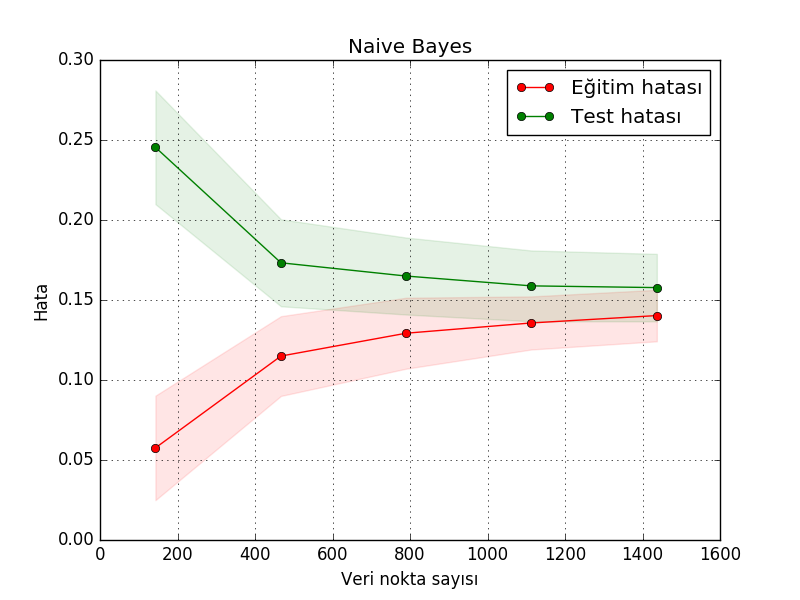
\includegraphics[width=30em]{biasvar_02.png}

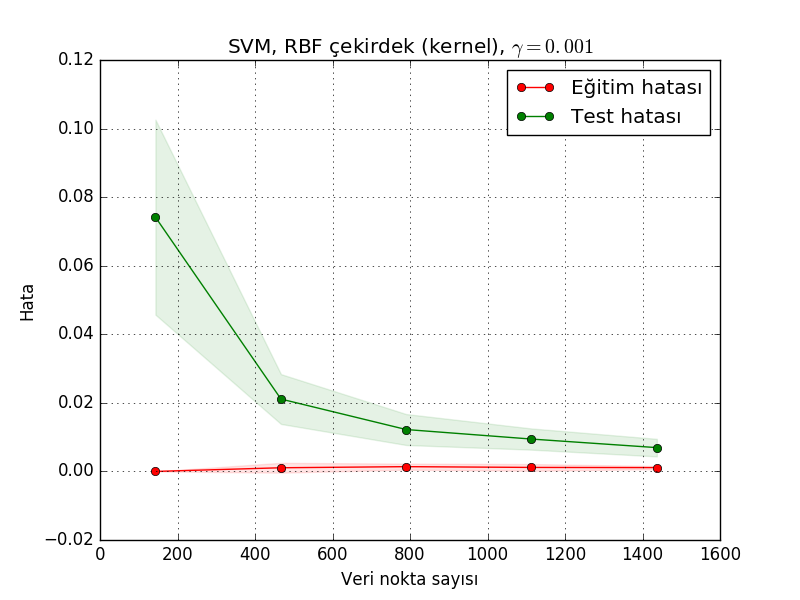
\includegraphics[width=30em]{biasvar_03.png}

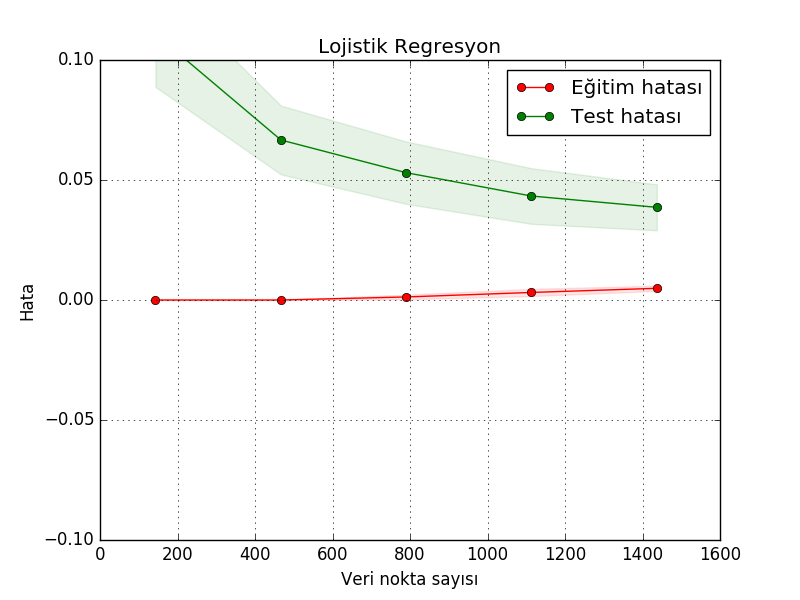
\includegraphics[width=30em]{biasvar_04.png}











\end{document}
